\documentclass[10pt]{beamer}

%~ \documentclass[10pt,handout]{beamer}   % uncomment for printable handouts (without animations)
%~ \usepackage{pgfpages}
%~ \pgfpagesuselayout{4 on 1}[a4paper,landscape,border shrink=5mm]

\usepackage[utf8]{inputenc}
\usepackage[czech]{babel}

\usepackage{amsmath,amsthm,amssymb,hyperref}
\usepackage{graphicx,color,tabularx,float,caption,subcaption,multirow}   % nicefrac

% magic: use both cline & czech
\makeatletter
\begingroup
\toks0=\expandafter{\@cline{#1}-{#2}\@nil}
\@ifpackageloaded{booktabs}{\toks2=\expandafter{\@@@cmidrule[{#1}-{#2}]{#3}{#4}}}{}
\catcode`-=\active
\edef\x{\gdef\unexpanded{\@cline#1-#2\@nil}{\the\toks0}}\x
\@ifpackageloaded{booktabs}{\edef\x{\gdef\unexpanded{\@@@cmidrule[#1-#2]#3#4}{\the\toks2}}\x}{}
\endgroup
\makeatother

%~ \newcommand{\Q}{\mathbb{Q}}
%~ \newcommand{\R}{\mathbb{R}}
%~ \newcommand{\Z}{\mathbb{Z}}
%~ \newcommand{\N}{\mathbb{N}}
%~ \newcommand{\primes}{\mathbb{P}}
%~ \newcommand{\GCD}{\mathsf{GCD}}
%~ \newcommand{\lcm}{\mathsf{lcm}}
%~ \renewcommand{\iff}{\Leftrightarrow}
\newcommand{\then}{\Rightarrow}
%~ \newcommand{\powerset}[1]{\mathcal{P} ( #1 )}
\newcommand{\GF}{\mathsf{GF}}

\let\phi\varphi
\let\epsilon\varepsilon

\theoremstyle{plain}
	\newtheorem{thm}{Teorém}[section]
	\newtheorem{lem}[thm]{Lemma}
	\newtheorem{tvr}[thm]{Tvrzení}
	\newtheorem*{dusl}{Důsledek}

\theoremstyle{definition}
	\newtheorem{defn}{Definice}[section]
	\newtheorem{prikl}[defn]{Příklad}
	%~ \newtheorem{exc}[example]{Exercise}

\theoremstyle{remark}
	\newtheorem{pzr}{Pozorování}[section]
	\newtheorem{pozn}[pzr]{Poznámka}

\usetheme{Malmoe}
\usecolortheme{rose}
\setbeamertemplate{blocks}[default]

\setbeamertemplate{section in toc}{\inserttocsectionnumber.~\inserttocsection}
\setbeamertemplate{subsection in toc}{\vspace{.3em}\hspace{1.2em}{\scriptsize\color{structure.fg}$\blacksquare$}~\inserttocsubsection\par}

\setbeamertemplate{itemize item}{\scriptsize\color{structure.fg}$\blacksquare$}
\setbeamertemplate{itemize subitem}{\tiny\color{structure.fg}$\blacksquare$}
\setbeamertemplate{itemize subsubitem}{\tiny\color{structure.fg}$\blacksquare$}
\setbeamertemplate{enumerate item}{\insertenumlabel.}
\setbeamertemplate{enumerate subitem}{\insertenumlabel.\insertsubenumlabel}
\setbeamertemplate{enumerate subsubitem}{\insertenumlabel.\insertsubenumlabel.\insertsubsubenumlabel}

%~ \setbeamercolor{frametitle}{bg=block title.bg}   % does not work without a block on the first slide ...
\setbeamercolor{frametitle}{parent=block body}
\setbeamercolor{frametitle}{fg=block title.fg}

\setbeamertemplate{navigation symbols}{
	\usebeamerfont{footline}
	\usebeamercolor[fg]{footline}
	\insertframenumber/\inserttotalframenumber
}

\setbeamertemplate{headline}{
	\begin{beamercolorbox}[ht=10pt]{section in head/foot}
		\vskip2pt\insertsectionnavigationhorizontal{\paperwidth}{}{\hskip0pt plus1filll}\vskip2pt
	\end{beamercolorbox}
	\begin{beamercolorbox}[ht=10pt]{subsection in head/foot}
		\vskip2pt\insertsubsectionnavigationhorizontal{\paperwidth}{}{\hskip0pt plus1filll}\vskip2pt
	\end{beamercolorbox}
}

\setbeamercovered{transparent=15}
%~ \setbeamercovered{highly dynamic}

%~ \setbeamertemplate{note page}[plain]
%~ \setbeameroption{show notes on second screen=right}   % pro zobrazení poznámek

% ======================================================================
%    S T A R T
% ======================================================================

\title[Analýza AES white-box schémat pomocí útoku postranním kanálem]{Analýza AES white-box schémat\\[.3em]pomocí útoku postranním kanálem}
\institute
{
	Katedra matematiky\\[.3em]
	FJFI, ČVUT
}
\author[Autor: Jakub Klemsa\qquad Školitel: prof. RNDr. Václav Matyáš, M.Sc., Ph.D.]{Autor: Jakub Klemsa\\[.3em]Školitel: prof. RNDr. Václav Matyáš, M.Sc., Ph.D.}
\date{\today}

\begin{document}

\frame{
	\titlepage
}

\frame{
	\tableofcontents
}

%~ \frame{   % průběžný obsahy
%~ \frametitle{Table of Contents}
%~ 	\tableofcontents[currentsection,currentsubsection,hideothersubsections,sectionstyle=show/shaded,]
%~ }


% ==============================================================================
% ===   I N G R E D I E N C E                                                ===
% ==============================================================================

\section{Ingredience}
\subsection{Advanced Encryption Standard (AES)}
\frame{
\frametitle{Advanced Encryption Standard (AES)}
	Symetrická bloková šifra
	%~ \begin{description}
		%~ \item[symetrická:] stejný klíč pro zašifrování i pro dešifrování\\(cf.\ asymetrická)
		%~ \item[bloková:] zpracovává vstup po blocích ($128$ bitů)\\(cf.\ proudová)
	%~ \end{description}
	\begin{itemize}
		\item standard vydaný NIST \cite[2001]{fips2001aes}
		\item dodnes považována za bezpečnou
	%~ \end{itemize}
	%~ \pause
%~ }
%~ 
%~ \frame{
%~ \frametitle{Konstrukce AES}
	%~ Varianta se $128$-bitovým klíčem
	%~ $128$-bitová varianta
		\pause
		\item $128$-bitová varianta
	%~ \begin{itemize}
		%~ \item $10$ rund, $4$ elementární operace
		%~ \item první mezivýsledky tvaru $S(m_i \oplus k_i)$, kde
		%~ \begin{description}
			%~ \item[$m_i$, $k_i$] \ldots\, $i$-tý byte zprávy $m$ resp.\ klíče $k$
			%~ \item[$\oplus$] \ldots\, operace XOR, bit po bitu
			%~ \item[$S$] \ldots\, nelineární bijekce (též SBox)
		%~ \end{description}
		\item {\bf mezivýsledky zranitelné}
	\end{itemize}
	%~ {\bf Mezivýsledky jsou zranitelné!}
}

\subsection{Od black-box k white-box modelu}
\frame{
\frametitle{Black-box model}
	Útočník má černou skříňku, která
	\begin{itemize}
		\item uchovává náhodný AES klíč
		\item zašifruje vloženou zprávu
		\item neunikne {\bf žádná} další informace
		\begin{itemize}
			\item mezivýsledky, doba šifrování, \ldots
		\end{itemize}
	\end{itemize}
	\pause
	Snaha útočníka: {\bf získat klíč}
	\begin{itemize}
		\item uhodnutý klíč snadno ověří
	\end{itemize}
}

\frame{
\frametitle{Gray-box model}
	%~ Black-box příliš idealizovaný
	Blíže realitě
	\begin{itemize}
		\item z hardwaru informace uniká
		\begin{itemize}
			\item spotřeba energie, EM záření, \ldots
		\end{itemize}
	\end{itemize}
	$\then$ útok postranním kanálem (dále)
}

\frame{
\frametitle{White-box model}
	Útočník vykonává šifrování
	\begin{itemize}
		\item vidí mezivýsledky
		\item může měnit hodnoty, instrukce, \ldots
		\item klíč musí zůstat utajen
	\end{itemize}
	\pause
	\begin{pzr}
		Odolnost k white-box $\then$ odolnost ke gray-box.
	\end{pzr}
}

\subsection{White-box AES (WBAES)}
\frame{
\frametitle{White-box AES (WBAES)}
	Představeno Chow et al.\ \cite[2002]{chow2002aes}
	\begin{itemize}
		\item algebraický útok (Billet et al.\ \cite[2004]{billet2004cryptanalysis})
	\end{itemize}
	\pause
	Skrývá mezivýsledky
	\begin{itemize}
		\item plně tabulková implementace
		\item tabulky obklopené náhodnými bijekcemi
		\item vhodně se vyruší $\then$ zachová funkcionalitu
		%~ \item zobrazení $F$ obklopeno náhodnými bijekcemi \ldots $H\circ F\circ G^{-1}$
		%~ \pause
		%~ \item po sobě jdoucí se vyruší\\$\ldots\underbrace{H_2\circ F_2\circ H_1^{-1}}_\textnormal{$n+1$. tabulka}\circ\underbrace{H_1\circ F_1\circ G_1^{-1}}_\textnormal{$n$. tabulka}\ldots$
		%~ \item při ošetření okrajů zachová funkcionalitu
	\end{itemize}
}

\subsection{Útok postranním kanálem (SCA)}
\frame{
\frametitle{Útok postranním kanálem (SCA) I}
	Kombinuje
	\begin{itemize}
		\item zranitelnost mezivýsledků
		\item únik informace v gray-box modelu (nazveme {\em stopa})
	\end{itemize}
	\pause
	Celá řada SCA
	\begin{itemize}
		\item přímé pozorování klíče (RSA)
		\item hádání klíče {\bf nezávisle po částech}
		\begin{itemize}
			\item hledání náznaků očekávaných mezivýsledků ve stopách
		\end{itemize}
	\end{itemize}
}

\frame{
\frametitle{Útok postranním kanálem (SCA) II}
	Příklad útoku proti AES
	\begin{itemize}
		\item prochází hodnoty $i$-tého bytu klíče
		\pause
		\begin{itemize}
			\item dělí stopy podle $j$-tého bitu očekávaného mezivýsledku
			\begin{itemize}
				\item nazveme {\em terč} (máme jich $8$)
				\item závisí na zprávě a klíči
			\end{itemize}
		\end{itemize}
		\pause
		\item max.\ rozdíl středních hodnot $\sim$ správný klíč
	\end{itemize}
	
	%~ \begin{itemize}
		%~ \pause
		%~ \item sběrnice přenáší mezivýsledky $S(m_i \oplus k_i)$
		%~ \pause
		%~ \item $8$ sond měřících napětí (stopa přísl.\ $m$)
		%~ \pause
		%~ \item hádám $i$-tý byte klíče $k_i^*$ a dělím stopy dle $j$-tého bitu $S(m_i \oplus k_i^*)$
		%~ \begin{itemize}
			%~ \item $j$-tý bit $S(m_i \oplus k_i^*)$ nazveme {\em terč} (máme jich $8$)
		%~ \end{itemize}
		%~ \pause
		%~ \item max.\ rozdíl středních hodnot stop $\sim$ správný klíč
	%~ \end{itemize}
	% vocaď
	%~ \pause
	%~ $\then$ stačí hádat byte po bytu!
	%~ \begin{itemize}
		%~ \item místo procházení $2^{128}$ možností jen $16\cdot256=2^{12}=4096$
	%~ \end{itemize}
}


% ==============================================================================
% ===   Ú T O K   N A   W H I T E - B O X   A E S                            ===
% ==============================================================================

\section{Útok na WBAES}
\subsection{Využití nástrojů SCA k útoku na WBAES}
\frame{
\frametitle{Využití nástrojů SCA k útoku na WBAES}
	%~ White-box implementace má být odolná na všechny SCA
	%~ \begin{itemize}
		%~ \item mezivýsledky schovány náhodnými bijekcemi
		%~ \item širší škála stop, hlavně adresy a obsah paměti
	%~ \end{itemize}
	%~ \pause
	\begin{pzr}[opakování]
		Odolnost k white-box $\then$ odolnost ke gray-box (tj.\ SCA).
	\end{pzr}
	\pause
	Bos et al.\ \cite[čvc.\ 2015]{bos2015differential}: SCA na white-box implementace
	\pause
	\begin{itemize}
		\item zlomili všechny veřejně dostupné
		\pause
		\item jen jedno tabulkové AES (Klinec \cite{klinec2013implementation})
		\begin{itemize}
			\item není zřejmé, kudy informace uniká
		\end{itemize}
		\pause
		\item paměťové stopy
		\begin{itemize}
			\item adresy čtení/zápisu
			\item obsah paměti
		\end{itemize}
	\end{itemize}
}

%~ \subsection{Postup útoku}
%~ \frame{
%~ \frametitle{Postup útoku I}
	%~ \begin{itemize}
		%~ \item získání paměťových stop
		%~ \begin{itemize}
			%~ \item poslední byte adresy nebo obsah
		%~ \end{itemize}
		%~ \item získání a vyfiltrování paměťových stop
		%~ \begin{itemize}
			%~ \item hodnoty konstantní napříč stopami
			%~ \item vizuální rozsah
		%~ \end{itemize}
	%~ \end{itemize}
%~ }
%~ 
%~ \frame[plain]{
	%~ \begin{figure}[h]
	%~ \begin{center}
		%~ 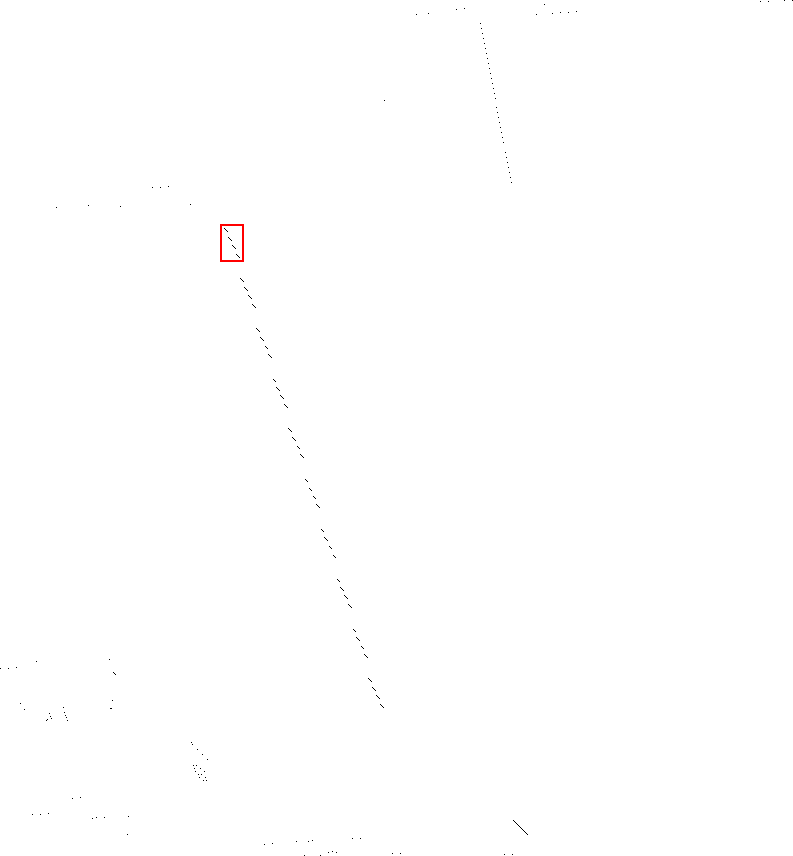
\includegraphics[height=\textheight]{../figures/memtrace/memtrace_emph.png}
	%~ \caption{Paměťová stopa běhu AES (část). První runda vyznačena červeně.}
	%~ \end{center}
	%~ \end{figure}
%~ }
%~ 
%~ \frame{
%~ \frametitle{Postup útoku II}
	%~ \begin{itemize}
		%~ \item spuštění vybraného SCA
		%~ \item ověření nalezeného klíče, případně opakujeme
		%~ \begin{itemize}
			%~ \item s více stopami,
			%~ \item s dalšími terči (dále)
		%~ \end{itemize}
	%~ \end{itemize}
%~ }

\subsection{Nové terče}
\frame{
%~ \frametitle{Nové terče I}
\frametitle{Nové terče}
	WBAES obklopuje mezivýsledky mj.\ náhodným lineárním zobrazením
	\begin{itemize}
		\item původní terče $\sim$ násobení mezivýsledku e.g. $(0,0,1,0,\;0,0,0,0)$
		\item nové terče $\sim$ násobení lib.\ nenulovým vektorem
	\end{itemize}
	$\then$ $255$ nových terčů
	%~ WBAES nerozliší, které tzv.\ {\em duální AES} je použito (Klinec \cite[2013]{klinec2013white})
	%~ \pause
	%~ \begin{itemize}
		%~ \item SBox -- afinní zobrazení \uv{inverze} v $\GF(2^8)$
		%~ \pause
		%~ \item v duálním AES libovolné invertibilní afinní
		%~ \pause
		%~ \item $S_{dual}(A) = p\cdot A' + q \mod{x^8+1}$
		%~ \begin{itemize}
			%~ \item $p$ nesoudělný s $x^8+1$
		%~ \end{itemize}
	%~ \end{itemize}
	%~ \pause
	%~ $\then$ první nové terče ($128$ různých)
	% vocaď
	%~ $\then$ první nové terče ({\em kolik různých?})
	%~ \pause
	%~ \begin{itemize}
		%~ \item vliv $q$: prohození $0$ a $1$, položíme $q=0$
		%~ \pause
		%~ \item vliv $p$: násobení $x\mod{x^8+1}$ $\sim$ cyklická rotace, uvaž.\ jen třídy
	%~ \end{itemize}
	%~ \pause
	%~ Celkem $128$ inv.\ $p$, $8$ ve třídě, $8$ terčů na každé $p$ $\then$ $128$ terčů
}

%~ \frame{
%~ \frametitle{Nové terče II}
	%~ Maticový zápis násobení$\mod{x^8+1}$
	%~ \begin{itemize}
		%~ \item cyklicky rotované řádky
		%~ \item lichý počet jedniček (invertibilita)
		%~ \item terč $\sim$ skalární součin řádku matice a $A'$
	%~ \end{itemize}
	%~ \pause
	%~ SBox následován náhodným lin.\ zobrazením
	%~ \begin{itemize}
		%~ \item použiju i řádky se sudým počtem jedniček
	%~ \end{itemize}
	%~ \pause
	%~ $\then$ další nové terče ($127$, bez $[0,\ldots,0]$), celkem $255$ terčů
%~ }

\section{Výsledky}
\subsection{Reprodukce výsledků Bos et al.}
\frame{
\frametitle{Reprodukce výsledků Bos et al.}
	Bos et al.\ -- útok na WBAES
	\begin{itemize}
		\item $8$ původních $+$ $8$ dalších terčů (jiný přístup)
		\item všech $16$ funguje
		\item reprodukujeme k porovnání s novými terči
	\end{itemize}
}

\frame[plain]{
	\begin{table}[H]
		\begin{center}
		\begin{tabular}{| c | r | r | r | r | r | r | r | r |}
	\hline
	\multirow{2}{*}{Byte} & \multicolumn{8}{c|}{Terče: bity orig.\ SBoxu} \\
	\cline{2-9}
	~ & 1. & 2. & 3. & 4. & 5. & 6. & 7. & 8. \\
	\hline
	1.&$\blacksquare$&55&90&$\blacksquare$&149&207&224&$\blacksquare$\\
	\hline
	2.&248&218&239&244&247&$\blacksquare$&251&247\\
	\hline
	3.&$\blacksquare$&212&$\blacksquare$&25&230&$\blacksquare$&99&$\blacksquare$\\
	\hline
	4.&$\blacksquare$&252&226&247&$\blacksquare$&255&241&252\\
	\hline
	5.&247&104&$\blacksquare$&225&229&$\blacksquare$&225&249\\
	\hline
	6.&252&255&$\blacksquare$&241&242&$\blacksquare$&4&255\\
	\hline
	7.&47&233&$\blacksquare$&228&$\blacksquare$&$\blacksquare$&$\blacksquare$&$\blacksquare$\\
	\hline
	8.&$\blacksquare$&253&253&$\blacksquare$&255&251&1&$\blacksquare$\\
	\hline
	9.&224&196&231&249&253&238&$\blacksquare$&253\\
	\hline
	10.&$\blacksquare$&$\blacksquare$&255&245&255&$\blacksquare$&234&$\blacksquare$\\
	\hline
	11.&245&$\blacksquare$&250&$\blacksquare$&190&255&236&$\blacksquare$\\
	\hline
	12.&254&255&$\blacksquare$&255&$\blacksquare$&$\blacksquare$&$\blacksquare$&$\blacksquare$\\
	\hline
	13.&241&$\blacksquare$&254&190&160&193&$\blacksquare$&$\blacksquare$\\
	\hline
	14.&235&$\blacksquare$&254&$\blacksquare$&255&2&$\blacksquare$&255\\
	\hline
	15.&$\blacksquare$&$\blacksquare$&246&195&255&$\blacksquare$&246&155\\
	\hline
	16.&252&255&254&$\blacksquare$&251&245&235&$\blacksquare$\\
	\hline
\end{tabular}
		\end{center}
	\caption{Pořadí správného kandidáta, $\blacksquare\sim 0$. Útok s~použitím $1024$ stop. Průměrně $2.9$ terčů z $8$ uspěje ($36\%$).}
	\end{table}
}

\frame[plain]{
	\begin{table}[H]
		\begin{center}
		\begin{tabular}{| c | r | r | r | r | r | r | r | r |}
	\hline
	\multirow{2}{*}{Byte} & \multicolumn{8}{c|}{Dalších $8$ terčů} \\
	\cline{2-9}
	~ & 1. & 2. & 3. & 4. & 5. & 6. & 7. & 8. \\
	\hline
	1.&207&$\blacksquare$&4&252&253&252&$\blacksquare$&$\blacksquare$\\
	\hline
	2.&233&255&252&$\blacksquare$&216&255&255&$\blacksquare$\\
	\hline
	3.&254&209&$\blacksquare$&$\blacksquare$&254&225&247&189\\
	\hline
	4.&37&$\blacksquare$&251&$\blacksquare$&$\blacksquare$&252&231&242\\
	\hline
	5.&244&$\blacksquare$&250&231&134&79&214&223\\
	\hline
	6.&$\blacksquare$&253&255&254&$\blacksquare$&$\blacksquare$&$\blacksquare$&2\\
	\hline
	7.&$\blacksquare$&248&187&255&209&$\blacksquare$&184&227\\
	\hline
	8.&$\blacksquare$&255&255&242&234&253&$\blacksquare$&255\\
	\hline
	9.&227&156&237&243&229&232&$\blacksquare$&$\blacksquare$\\
	\hline
	10.&$\blacksquare$&158&1&$\blacksquare$&253&$\blacksquare$&$\blacksquare$&$\blacksquare$\\
	\hline
	11.&248&$\blacksquare$&241&254&251&45&255&1\\
	\hline
	12.&$\blacksquare$&251&254&255&236&255&$\blacksquare$&254\\
	\hline
	13.&205&4&191&30&$\blacksquare$&$\blacksquare$&240&255\\
	\hline
	14.&$\blacksquare$&231&246&$\blacksquare$&248&253&$\blacksquare$&$\blacksquare$\\
	\hline
	15.&221&250&1&$\blacksquare$&223&$\blacksquare$&1&225\\
	\hline
	16.&255&$\blacksquare$&229&254&$\blacksquare$&255&254&253\\
	\hline
\end{tabular}
		\end{center}
	\caption{Pořadí správného kandidáta, $\blacksquare\sim 0$. Útok s~použitím $1024$ stop. Průměrně $2.4$ terčů z $8$ uspěje ($30\%$).}
	\end{table}
}

\subsection{Výsledky použití všech $255$ terčů}
\frame{
\frametitle{Výsledky použití všech $255$ terčů}
	Nagenerováno $8$ instancí WBAES tabulek
	\begin{itemize}
		\item $255$ terčů pro každý ze $16$ bytů klíče a každou z $8$ instancí
		\begin{itemize}
			\item $32\,640$ útoků
			\item doba běhu desítky hodin
		\end{itemize}
		\pause
		\item globální úspěšnost $29\%$
		\begin{itemize}
			\item silní kandidáti -- rozdíl na druhého $>10\%$
			\item úsp.\ $25\%$   % [1019, 1000, 978, 1008, 986, 1006, 1019, 999].print_stats([:mean,:dev,:median,:sum])
		\end{itemize}
	\end{itemize}
}

\subsection{Rozložení úspěšnosti terčů}
\frame{
\frametitle{Rozložení úspěšnosti terčů I}
	Mnoho terčů, málo měření (každý alespoň jednou úspěšný)
	\begin{itemize}
		\item shlukování terčů -- může jen vyvrátit uniformitu
		\begin{itemize}
			\item cyklické rotace vektoru
			\item hlubší význam v konstrukci
		\end{itemize}
	\end{itemize}
	\begin{figure}[h]
	\begin{center}
		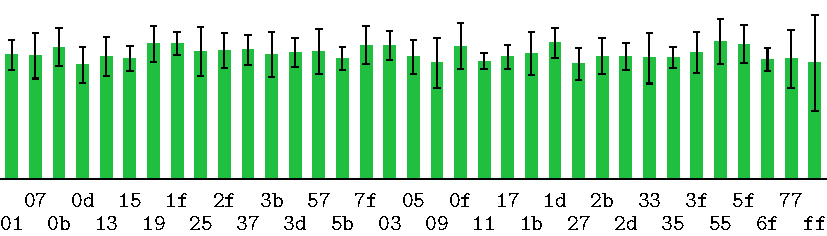
\includegraphics[width=\textwidth]{../figures/leak_target/leak_target_unicolor.pdf}
	%~ \caption{Úspěšnost terčů podle invertibility původního $p$: zeleně invertibilní, cihlově neinvertibilní. Pro méně než $8$ terčů na $p$ jsou výsledky přeškálovány.}
	\caption{Úspěšnost shluků terčů, hexadecimální zápis reprezentanta.}
	\end{center}
	\end{figure}
}

\frame{
\frametitle{Rozložení úspěšnosti terčů II}
	Fixované $4$ bity vektoru (maskami {\tt 0xf0}, {\tt 0x0f})
	%~ \begin{itemize}
		%~ \item shlukování terčů -- cyklické rotace vektoru
		%~ \item barvy -- vychází z kontrukce, jen ilustrační
	%~ \end{itemize}
	\begin{figure}[h]
	\begin{center}
		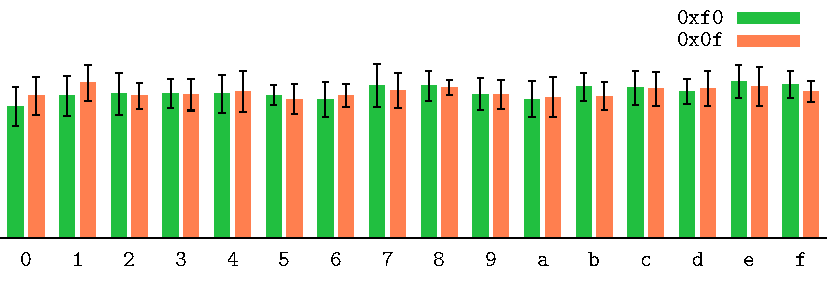
\includegraphics[width=\textwidth]{../figures/leak_target_other/leak_0x0f_0xf0.pdf}
	%~ \caption{Úspěšnost terčů podle invertibility původního $p$: zeleně invertibilní, cihlově neinvertibilní. Pro méně než $8$ terčů na $p$ jsou výsledky přeškálovány.}
	\caption{Úspěšnost shluků terčů, hexadecimální zápis fixovaných bitů.}
	\end{center}
	\end{figure}
}

\subsection{Útok \uv{naslepo}}
\frame{
\frametitle{Útok \uv{naslepo}}
	Znali jsme klíč, úskalí útoku \uv{naslepo}
	\begin{itemize}
		\item falešní kandidáti
		\begin{itemize}
			\item rekordní rozdíl na druhého téměř $35\%$
			\item ten samý se málokdy opakuje
		\end{itemize}
		\item průměrný rozdíl správných $34\%$
		\begin{itemize}
			\item klesá s počtem stop
		\end{itemize}
	\end{itemize}
	\pause
	Návrh
	\begin{itemize}
		\item menší počet stop a více terčů
		\item sčítání relativních rozdílů na druhého
		\begin{itemize}
			\item hranice pro započítání ($10\%$)
			\item hranice pro skončení ($75\%$)
		\end{itemize}
	\end{itemize}
	$\then$ zlomilo všechny instance (snad zlomí) %!% ověřit
}

%!% přesun z budoucí práce, něco se povedlo:
%~ \item reprodukoval jsem výsledky Bos et al.
%~ \item rozšířil jsem útok ze $16$ na $255$ terčů
%~ \item sjednotil jsem 
%~ \item identifikoval jsem mezivýsledek, ze kterého uniká informace
%~ \item odůvodnil jsem, který prvek konstrukce WBAES je zranitelný

\section{Budoucí práce}
\frame{
\frametitle{Budoucí práce I}
	Nedořešené otázky
	\begin{itemize}
		\item ze které tabulky WBAES dochází k úniku
		\begin{itemize}
			\item $3$ nefungující způsoby
			\begin{itemize}
				\item $2$ způsoby s debuggerem
				\item útok na indexy tabulek
			\end{itemize}
		\end{itemize}
		\item jak útok teoreticky podložit
		\begin{itemize}
			\item proč se správný kandidát propadá na poslední místa
		\end{itemize}
		%~ \item proč z pozice $3$ ve stopě neuniká informace
		%~ \item \ldots
	\end{itemize}
}

\frame{
\frametitle{Budoucí práce II}
	Úspěšnost podle pozice ve stopě
	\begin{itemize}
		\item místo úniku -- max.\ rozdíl středních hodnot stop
	\end{itemize}
	\begin{figure}[h]
	\begin{center}
		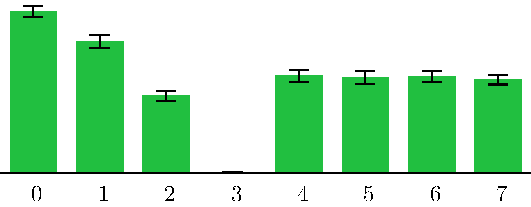
\includegraphics[width=.65\textwidth]{../figures/leak_bit/leak_bit.pdf}
	\caption{Průměrná úpěšnost a její směrodatná odchylka napříč instancemi podle pozice bitu v rámci bytu ve stopě.}
	\end{center}
	\end{figure}
}

\section*{Literatura}
\frame[allowframebreaks=0.95]{
%~ \frame{
\frametitle{Literatura}
	\bibliography{../biblio}{}
	\bibliographystyle{plain}
}

\end{document}